\documentclass{ximera}

\input{../../preamble.tex}

\author{Kenneth Berglund}

\begin{document}
\begin{exercise}

You and your friend decide to have a bike race. Your speed is 16 kilometers per hour, and your friend's is 20 kilometers per hour. Your friend is faster than you are, so they give you a head start of 2 kilometers.

Let $f(x)$ be a linear function expressing the distance (in kilometers) you travel, and $g(x)$ be a linear function expressing the distance (in kilometers) your friend travels. 

\begin{enumerate}
\item One of the following graphs represents $f(x)$ and the other represents $g(x)$.

\begin{image}
\begin{tikzpicture}
    \begin{axis}[title={Graph $A$},xmin=-1,xmax=3,ymin=-1,ymax=50,minor xtick=,
minor ytick=,xtick={0,1/2,...,3},ytick={0,10,...,50}]
        \addplot{20*x} node{Graph $A$};
    \end{axis}
    
\end{tikzpicture}
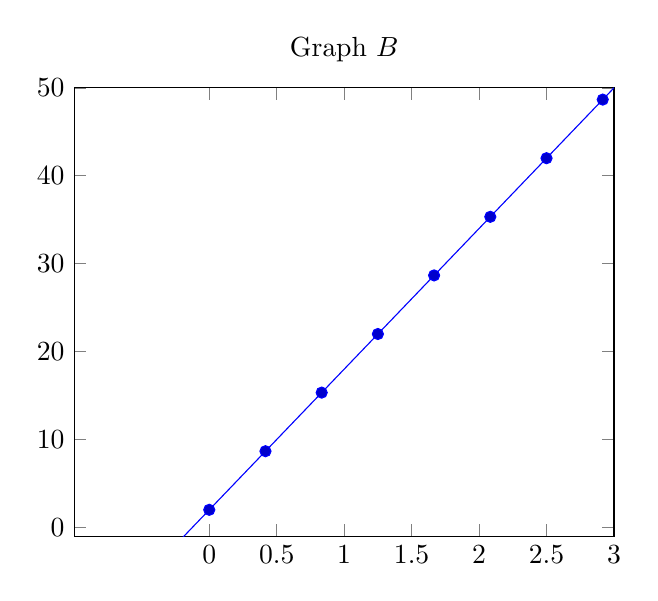
\begin{tikzpicture}
    \begin{axis}[title={Graph $B$},xmin=-1,xmax=3,ymin=-1,ymax=50,minor xtick=,
minor ytick=,xtick={0,1/2,...,3},ytick={0,10,...,50}]
        \addplot{16*x + 2} node{Graph $B$};
    \end{axis}
\end{tikzpicture}
\end{image}


The graph representing $f(x)$ is
\begin{multipleChoice}
\choice{Graph $A$.}
\choice[correct]{Graph $B$.}
\end{multipleChoice}


\item A linear equation for the distance you travel is $f(x) = \answer{16x + 2}$.

\item A linear equation for the distance your friend travels is $g(x) = \answer{20x}$.

\item If the race is 5 kilometers long, who will win?
\begin{multipleChoice}
\choice[correct]{You}
\choice{Your friend}
\choice{It will be a tie}
\end{multipleChoice}

\item If the race is 10 kilometers long, who will win?
\begin{multipleChoice}
\choice{You}
\choice{Your friend}
\choice[correct]{It will be a tie}
\end{multipleChoice}

\item If the race is 20 kilometers long, who will win?
\begin{multipleChoice}
\choice{You}
\choice[correct]{Your friend}
\choice{It will be a tie}
\end{multipleChoice}



	
\end{enumerate}

\end{exercise}
\end{document}